\section{PROJECT DETAILS}

This section describes the proposed VERACISM project in detail, from its core design to its operational workflow. It explains how existing ISM systems interact with the platform, how reports are processed, stored, and verified, and how stakeholders access these capabilities. It also highlights the security, integrity, and governance features that distinguish VERACISM from existing alternatives.

    \subsection{Overview}
       \begin{figure}[H]
        \centering
        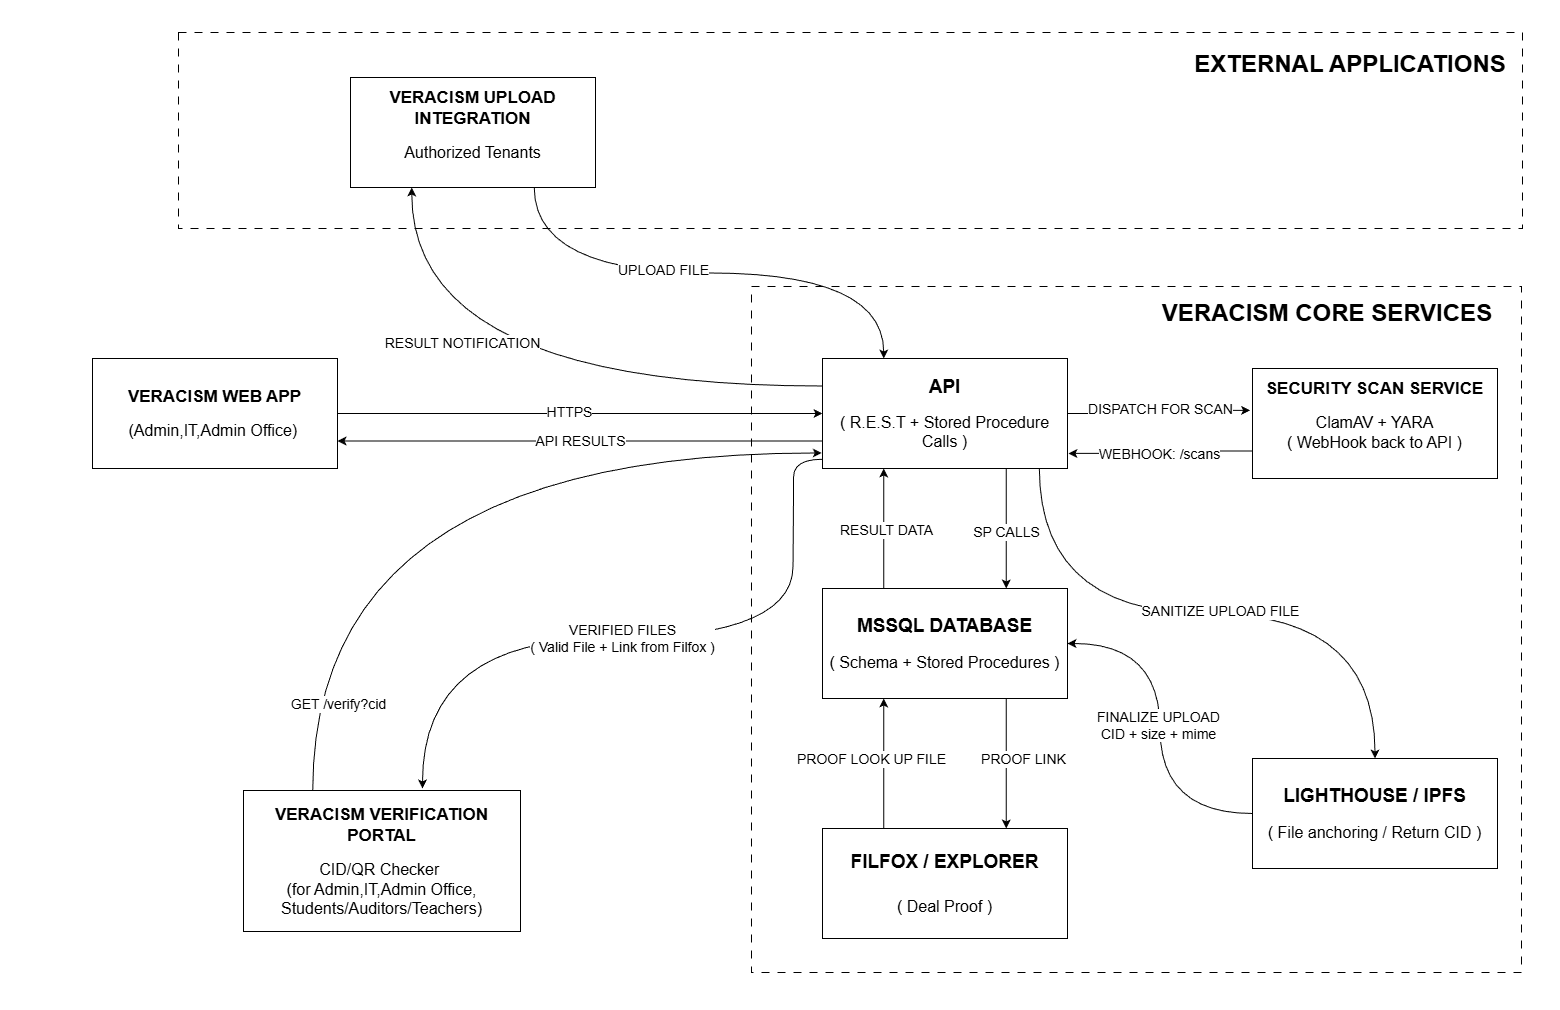
\includegraphics[height=0.45\textheight,keepaspectratio]{Texfiles/images/VERACISM SYSTEM DIAGRAM.png}
        \caption{System Structure}
        \label{fig:veracism-structure}
       \end{figure}
    VERACISM (Verifiable Academic Records for ISM) is a permanent, decentralized
    storage and verification service for finalized academic and administrative reports
    of International School Manila. Existing ISM systems generate reports and submit
    them through a secure \texttt{.NET~8} Web API, where each file is scanned for
    malware, validated, hashed with SHA-256, and stored via Lighthouse on IPFS with
    Filecoin-backed deals. The system issues a unique Content Identifier (CID) for
    each report and provides a web-based verification portal so internal and external
    stakeholders can independently confirm the integrity and authenticity of reports
    using CIDs or QR codes, without relying solely on ISM-hosted storage.

    \clearpage
    \subsection{Project Framework}
        \begin{figure}[H]
            \centering
            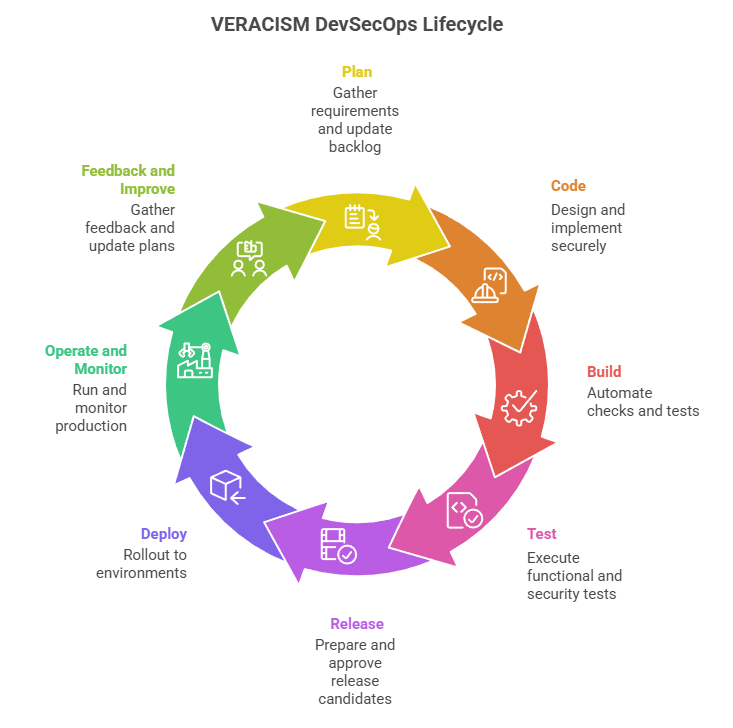
\includegraphics[height=0.45\textheight,keepaspectratio]{Texfiles/images/Veracism- DevSecOps.png}
            \caption{DevSecOps Lifecycle}
            \label{fig:veracism-devsecops}
        \end{figure}
    The VERACISM project follows a DevSecOps lifecycle adopted by the ISM development
team. Security is built into every phase, and the cycle repeats continuously. When
problems are found (functional issues, NFR gaps, or security findings), work loops
back to the planning and requirements stage instead of being treated as a one-time
activity.

The main DevSecOps phases for VERACISM are:

\begin{enumerate}
    \item \textbf{Plan (Information gathering and requirements)} \\
    Collect business needs, technical constraints, and security requirements from ISM
    stakeholders. Update the backlog with new features, risks, and compliance needs.

    \item \textbf{Code (Secure design and implementation)} \\
    Design and implement features with security in mind:
    hybrid architecture, RBAC/ABAC, immutable audit logging in MSSQL, and decentralized
    storage on IPFS/Filecoin for durability and verifiability. Apply secure coding
    practices and peer review.

    \item \textbf{Build (Automated checks)} \\
    Use CI pipelines to compile and package the .NET and front-end components. Run
    automated unit tests, static analysis, dependency checks (for example, Snyk or ISM
    equivalent), and basic security checks on every build.

    \item \textbf{Test (Functional, NFR, and security)} \\
    Execute functional tests, non-functional tests (performance, reliability, usability),
    and security tests including VAPT in alignment with ISM VAPT Guidelines. Test
    specifically for common OWASP Top 10 risks such as broken access control, injection,
    authentication failures, and logging/monitoring gaps.

    \item \textbf{Release (Approval and hardening)} \\
    Prepare release candidates with documented changes, risk assessments, and security
    results. Ensure that critical and high findings are addressed or formally
    risk-accepted according to ISM policy before promotion.

    \item \textbf{Deploy (Controlled rollout)} \\
    Deploy VERACISM to Dev, UAT, and Production using automated, repeatable pipelines.
    Apply hardened configuration, secret management, and environment-specific settings
    under ISM operational standards.

    \item \textbf{Operate and Monitor} \\
    Run VERACISM in production with immutable audit trails, structured logging, and
    health monitoring. Use dashboards and alerts to detect anomalies, performance issues,
    and security events.

    \item \textbf{Feedback and Improve} \\
    Incidents, test failures, monitoring alerts, and user feedback are fed back into the
    Plan phase. Requirements, designs, and controls are updated, and a new DevSecOps
    cycle starts. This repeating loop continues throughout the life of the VERACISM
    platform.
\end{enumerate}

\clearpage

\subsection{Materials/Technologies Used}
The implementation of VERACISM relies on the following key materials and
technologies:
\begin{itemize}
    \item \textbf{Application Backend:} \texttt{.NET~8} Web API hosted on ISM-controlled
          Linux or Windows servers or containers.
    \item \textbf{Database Layer:} Microsoft SQL Server (MSSQL~2019 or later) for
          tenant-aware metadata storage and immutable audit event records.
    \item \textbf{Decentralized Storage:} Lighthouse service for writing files to IPFS with
          Filecoin-backed deals, plus access to public IPFS gateways and a Filecoin
          explorer (e.g., Filfox) for external evidence of storage.
    \item \textbf{Security Tooling:} ClamAV and YARA rules for malware scanning; MIME
          type and file size validation; SHA-256 hashing for integrity checking.
    \item \textbf{Web Front-end:} Single-page application built using Angular or React
          with TypeScript, providing both the internal console and public verification
          portal.
    \item \textbf{Access Control and Identity:} Integration with ISM identity systems to
          support role-based and attribute-based access control for staff, service
          accounts, and other user classes.
    \item \textbf{Monitoring and Operations:} Existing ISM monitoring and logging
          systems for health checks, CID availability and latency checks, and alerting.
    \item \textbf{Verification Aids:} QR code generation and CID-based lookup features
          to support fast, user-friendly verification of report authenticity.
\end{itemize}

% --- short summary table (not compressed) ---
\begin{table}[H]
  \centering
  \smalltable
  \footnotesize

  {%
  \setlength{\tabcolsep}{8pt}% horizontal padding
  \renewcommand{\arraystretch}{1.4}% vertical padding

  \begin{tabular}{|>{\raggedright\arraybackslash}p{0.27\textwidth}|
                  >{\raggedright\arraybackslash}p{0.30\textwidth}|
                  >{\raggedright\arraybackslash}p{0.30\textwidth}|}
    \hline
    \textbf{Component} & \textbf{Main Technologies} & \textbf{Role in VERACISM} \\
    \hline\hline
    Backend and database &
    \texttt{.NET~8} Web API, MSSQL~2019+ &
    Coordinate uploads, apply policies, and store metadata and audit events. \\
    \hline
    Decentralized storage layer &
    Lighthouse, IPFS, Filecoin, public gateways, Filfox &
    Provide content-addressed, durable storage and public evidence of persistence. \\
    \hline
    Security and integrity tools &
    ClamAV, YARA, MIME/size validation, SHA-256 hashing &
    Block malicious files and generate cryptographic proofs of file integrity. \\
    \hline
    User-facing interfaces &
    Angular/React SPA, QR codes, CID lookup tools &
    Expose internal console and public verification portal for staff and external verifiers. \\
    \hline
    Identity, access, and operations &
    ISM identity systems, RBAC/ABAC, existing monitoring and logging stack &
    Control who can act on reports and keep the system observable and supportable. \\
    \hline
  \end{tabular}
  }% end local spacing changes

  \captionsetup{type=table}
  \caption{Summary of materials and technologies used in VERACISM}
  \label{table:materials-technologies-summary}
\end{table}

Table~\ref{table:materials-technologies-summary}, VERACISM combines a conventional enterprise stack (\texttt{.NET~8}, MSSQL, and ISM-managed servers) with decentralized storage (Lighthouse, IPFS, and Filecoin) and layered security tooling (ClamAV, YARA, and SHA-256 hashing). The web front-end, identity integration, and monitoring stack ensure that these components work together as one operational system that is verifiable from the outside yet remains manageable within ISM’s existing infrastructure.

\clearpage

    \subsection{System Design}
    The system design of VERACISM is guided by a clear set of functional and
    non-functional requirements and is supported by standard design models
    (use case, sequence, data model, and deployment diagrams). This section
    summarizes how the system is expected to behave and how the data is
    structured.

    \paragraph{Functional requirements.}
    At a high level, the main functional requirements are:
    \begin{itemize}
        \item \textbf{Encrypted Report file upload:} The system accepts report files (PDF,DOCS,DOCX) and
        their metadata from authorized ISM applications through a secure API.
        Valid, authenticated uploads are stored in temporary storage with a
        tracking identifier. Invalid, oversized, or unauthorized uploads are
        rejected with clear errors.

        \item \textbf{Malware scanning and file validation.} Every uploaded
        file is scanned for malware and checked for type and size before it is
        accepted into the permanent storage workflow. Files that fail scanning
        or validation are never stored.

        \item \textbf{Hashing and CID generation.} For each accepted file,
        the system computes a SHA-256 hash and generates or records the
        associated Content Identifier (CID). The hash and CID are treated as
        the source of truth for later verification.

        \item \textbf{Decentralized storage.} The system sends accepted
        report files to Lighthouse for storage on IPFS with Filecoin-backed
        deals and records the returned CID and storage details.

        \item \textbf{Metadata storage and immutable audit trail.} Report
        metadata and audit events are stored in MSSQL using a tenant-aware
        structure. Metadata includes at least the source report identifier,
        student identifier, term, academic level, file hash, CID, upload time,
        and producing system. Audit events record who or what acted, what
        action occurred, the timestamp, and the outcome. Audit events cannot
        be edited or deleted through normal interfaces.

        \item \textbf{Role-based and attribute-based access control.} Access
        to administrative functions and report retrieval is controlled using
        RBAC and ABAC rules. Staff and service accounts only see and perform
        operations they are allowed to use.

        \item \textbf{Verification portal and CID/QR verification.} The
        system provides a public verification portal where any user can submit
        a CID or scan a QR code to check if a report exists, confirm its hash,
        and see whether the stored file still matches the original.

        \item \textbf{Internal console and report search.} Authorized ISM
        staff can search reports by student, term, report identifier, or other
        metadata, view report details, and inspect audit history through an
        internal console.

        \item \textbf{Health monitoring and storage checks.} Scheduled jobs
        check CID availability, deal status, and retrieval latency. If thresholds
        are breached, the system logs events and raises alerts through ISM
        monitoring tools. Health status is shown on an operator dashboard.

        \item \textbf{Configuration and key management.} Configuration
        values and secrets (such as Lighthouse tokens and API keys) are
        centrally managed. Secrets are stored in a secure secret management
        solution and are never stored in plain text in source control. Changes
        to keys and critical configuration are logged.
    \end{itemize}

    \paragraph{Non-functional requirements.}
    The main non-functional requirements are:

    \begin{itemize}
        \item \textbf{Performance.} The upload API should respond within
        about two seconds for accepted files under normal load (after network
        arrival). The verification portal should respond within about three
        seconds for successful CID checks. The system should handle at least
        one hundred concurrent verification requests without unacceptable
        slowdown.

        \item \textbf{Security.} All traffic uses HTTPS with current TLS
        versions. Passwords and secrets are never logged. All external
        interfaces apply input validation and output encoding. Regular
        vulnerability scans are performed, and no critical or high findings
        are left unresolved beyond agreed timelines.

        \item \textbf{Availability and reliability.} Core upload and
        verification functions should achieve monthly uptime of at least
        99.5\%. Recovery time and recovery point objectives are defined for
        the MSSQL data so that service can be restored and data loss is kept
        within acceptable limits.

        \item \textbf{Usability.} Verification results use clear language
        and avoid protocol jargon. The user interface follows ISM design and
        accessibility guidelines and aligns with WCAG~2.2 where applicable.
        QR-based verification should be easy to use on mobile devices without
        zooming or horizontal scrolling.

        \item \textbf{Maintainability and supportability.} The codebase
        follows standard \texttt{.NET} structure with a clear separation of
        concerns. The front-end is a single-page application (SPA) built using
        Angular or React with TypeScript and follows a component-based
        structure and ISM coding guidelines. Configuration for Dev, UAT,
        and Prod is externalized and documented, and runbooks exist for
        deployment, incident response, backup/restore, and routine
        maintenance.

        \item \textbf{Audit and compliance.} All access to reports and
        configuration changes is logged and searchable. Audit reports can be
        exported in formats suitable for auditors (for example, CSV or PDF).
        The system retains the data needed to prove integrity and provenance
        of reports for the required retention period.
    \end{itemize}

    \clearpage
\subsection{Use case diagram}

% Pair 1
    \begin{figure}[H]
        \centering
        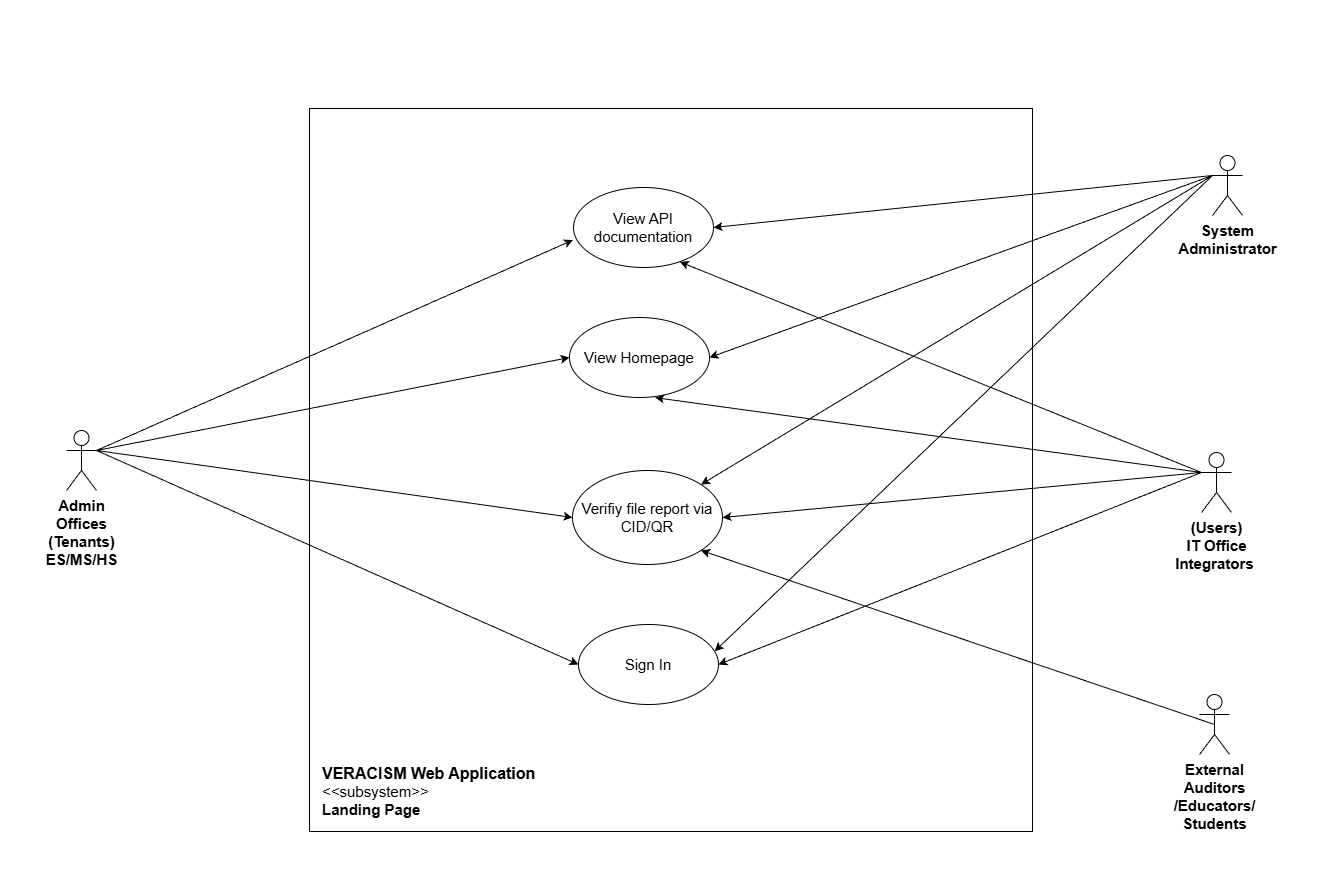
\includegraphics[height=0.43\textheight,keepaspectratio]{Texfiles/images/Use Case/Landing Page.png}
        \caption{Use Case Diagram - Landing Page}
        \label{fig:usecaseLandingPage-diagram}
    \end{figure}

    \begin{figure}[H]
        \centering
        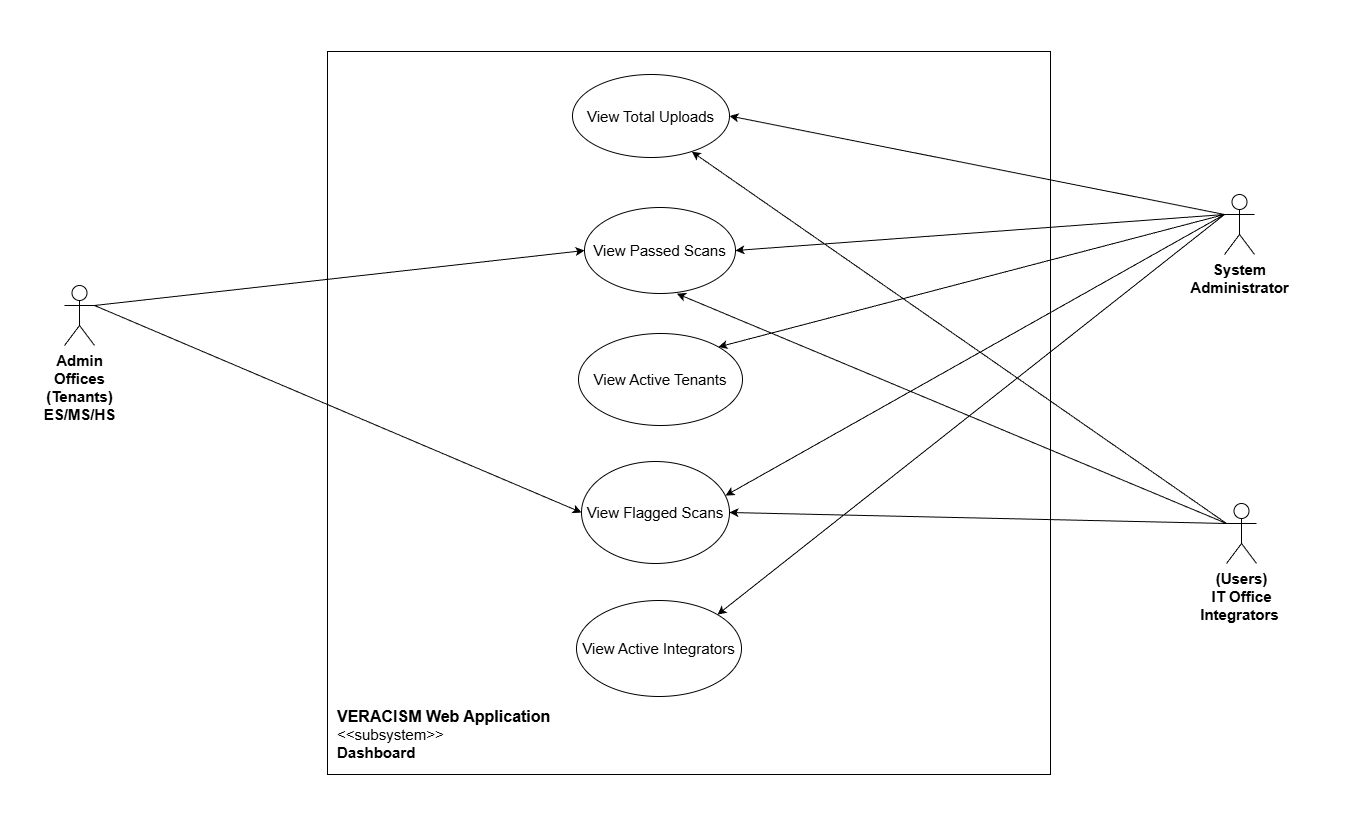
\includegraphics[height=0.43\textheight,keepaspectratio]{Texfiles/images/Use Case/Dashboard.png}
        \caption{Use Case Diagram - Dashboard}
        \label{fig:usecaseDashboard-diagram}
    \end{figure}

    \clearpage
    % Pair 2
    \begin{figure}[H]
        \centering
        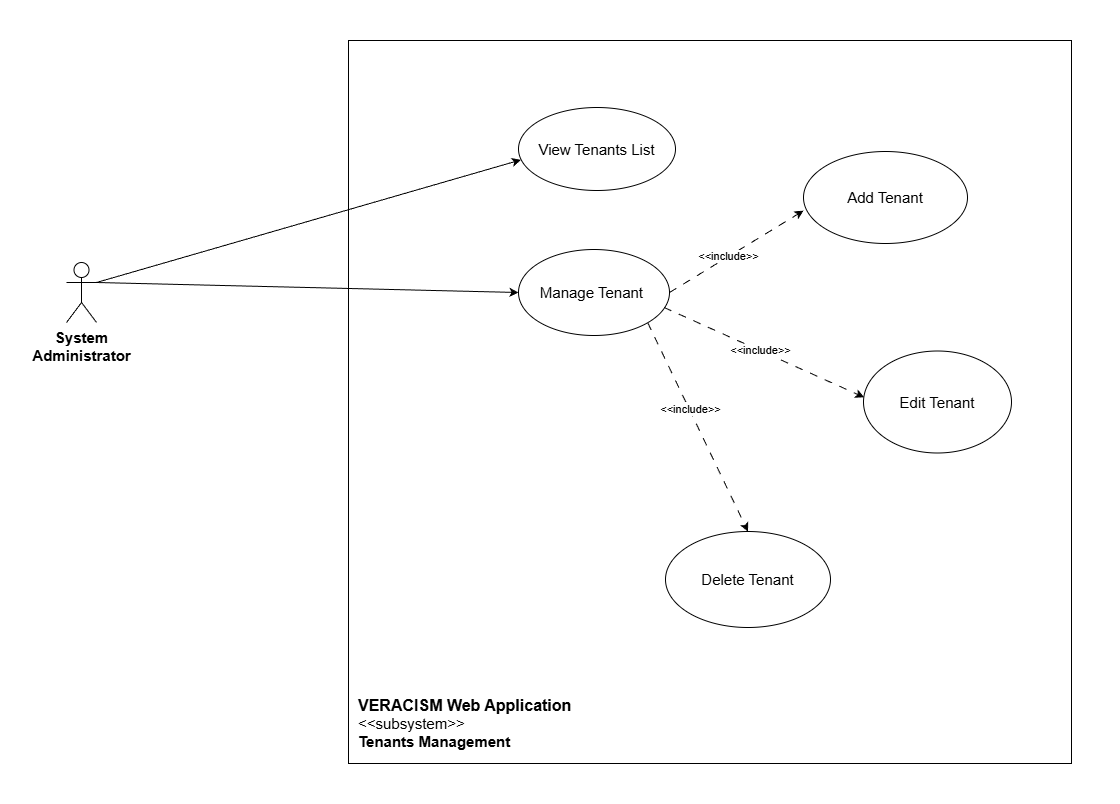
\includegraphics[height=0.43\textheight,keepaspectratio]{Texfiles/images/Use Case/Tenants Management.png}
        \caption{Use Case Diagram - Tenants Management}
        \label{fig:usecaseTenantsManagement-diagram}
    \end{figure}

    \begin{figure}[H]
        \centering
        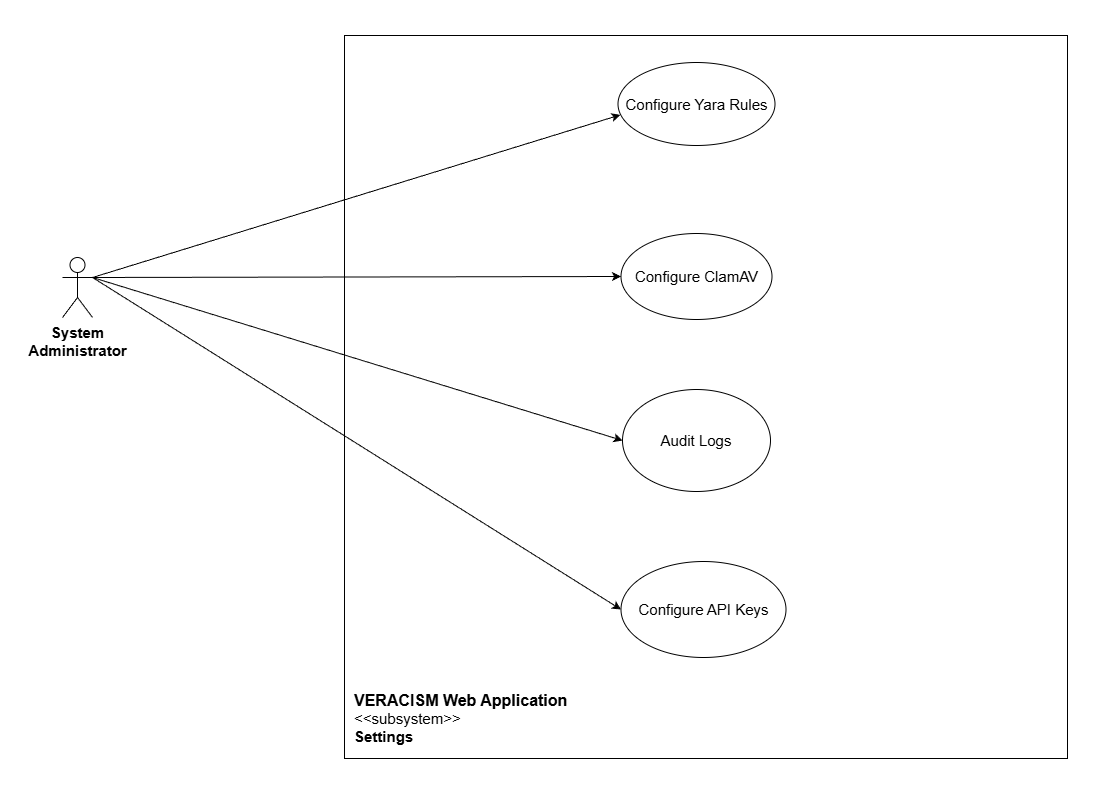
\includegraphics[height=0.43\textheight,keepaspectratio]{Texfiles/images/Use Case/Settings.png}
        \caption{Use Case Diagram - Settings}
        \label{fig:usecaseSettings-diagram}
    \end{figure}

    \clearpage
    % Pair 3
    \begin{figure}[H]
        \centering
        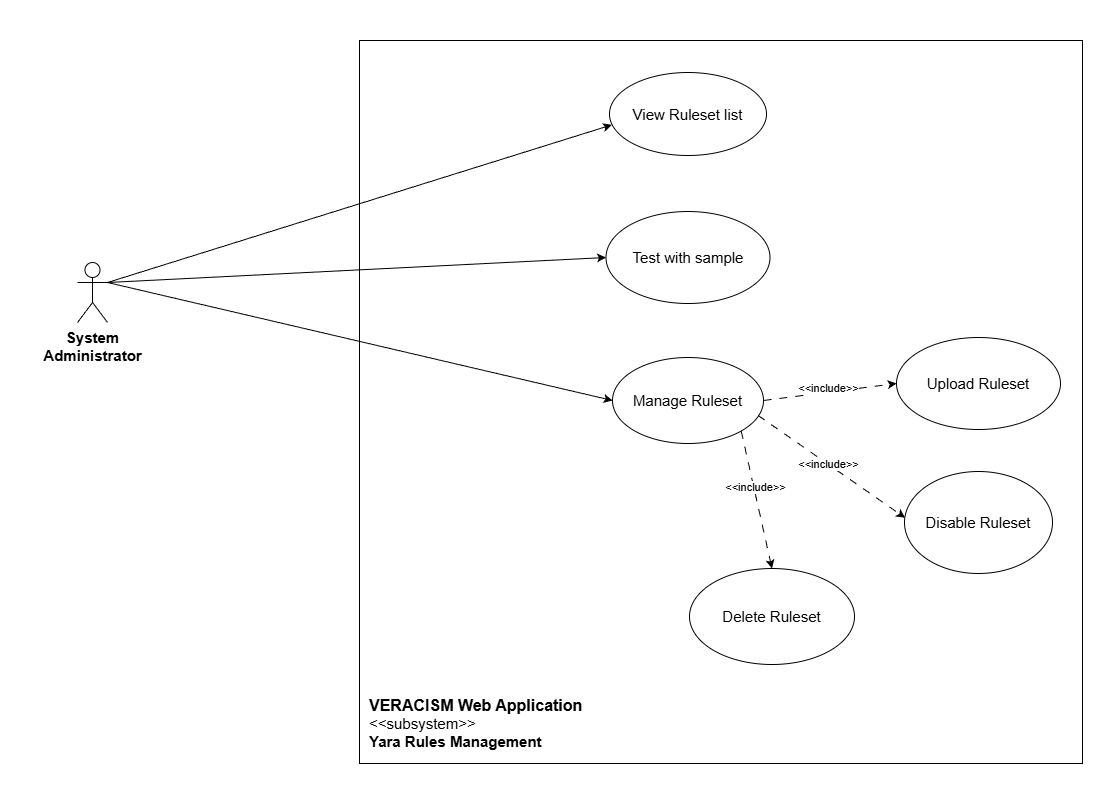
\includegraphics[height=0.43\textheight,keepaspectratio]{Texfiles/images/Use Case/Yara Rules Management.png}
        \caption{Use Case Diagram - Yara Rules Management}
        \label{fig:usecaseYaraRulesManagement-diagram}
    \end{figure}

    \begin{figure}[H]
        \centering
        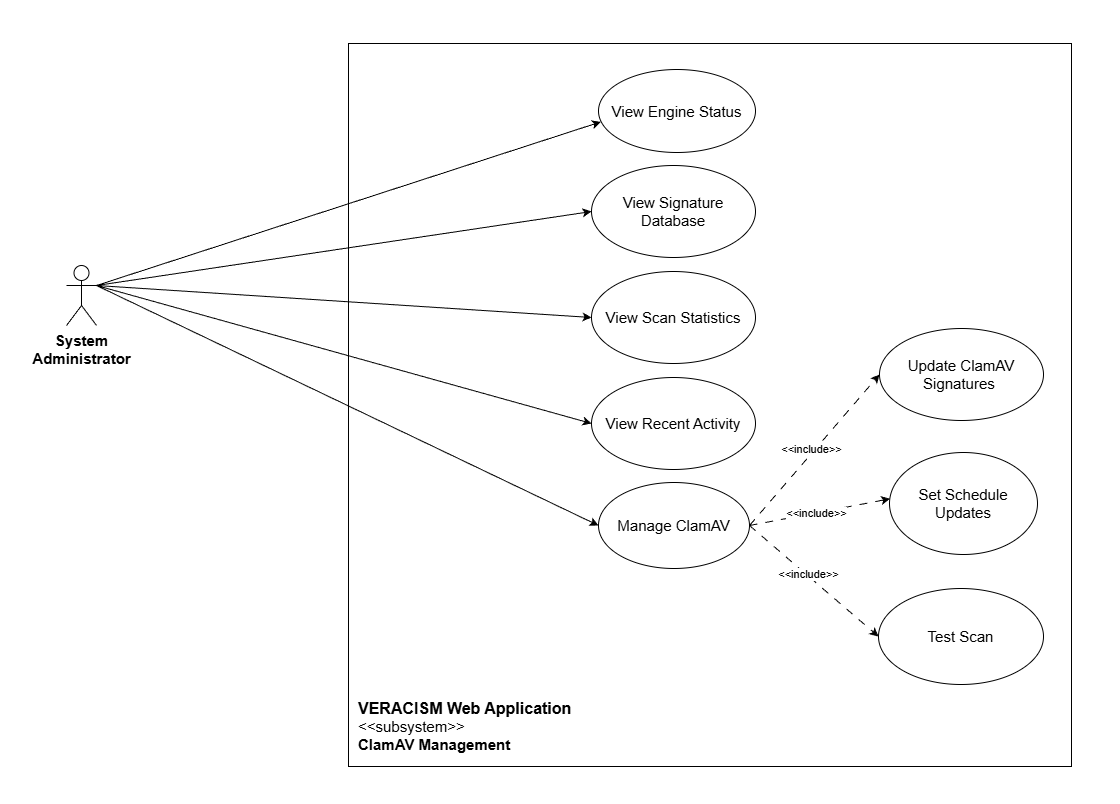
\includegraphics[height=0.43\textheight,keepaspectratio]{Texfiles/images/Use Case/ClamAV Management.png}
        \caption{Use Case Diagram - ClamAV Management}
        \label{fig:usecaseClamAVManagement-diagram}
    \end{figure}

    \clearpage
    % Pair 4
    \begin{figure}[H]
        \centering
        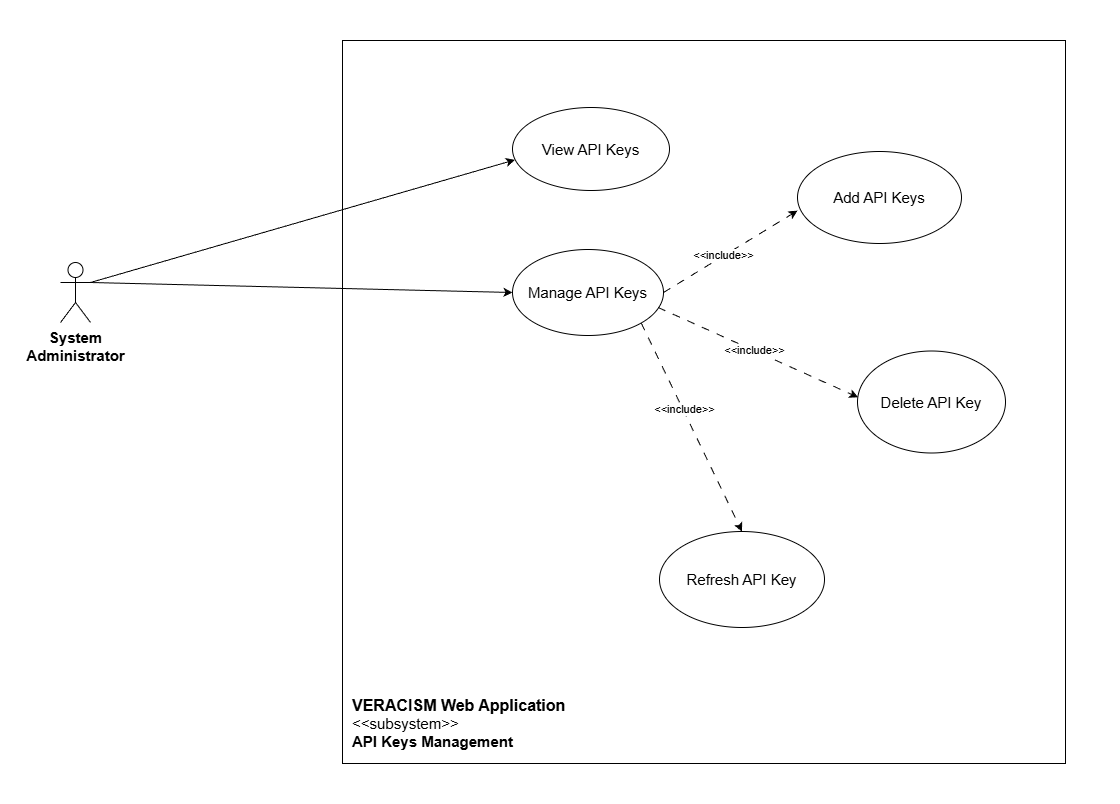
\includegraphics[height=0.43\textheight,keepaspectratio]{Texfiles/images/Use Case/API Keys Management.png}
        \caption{Use Case Diagram - API Keys Management}
        \label{fig:usecaseAPIKeysManagement-diagram}
    \end{figure}

    \begin{figure}[H]
        \centering
        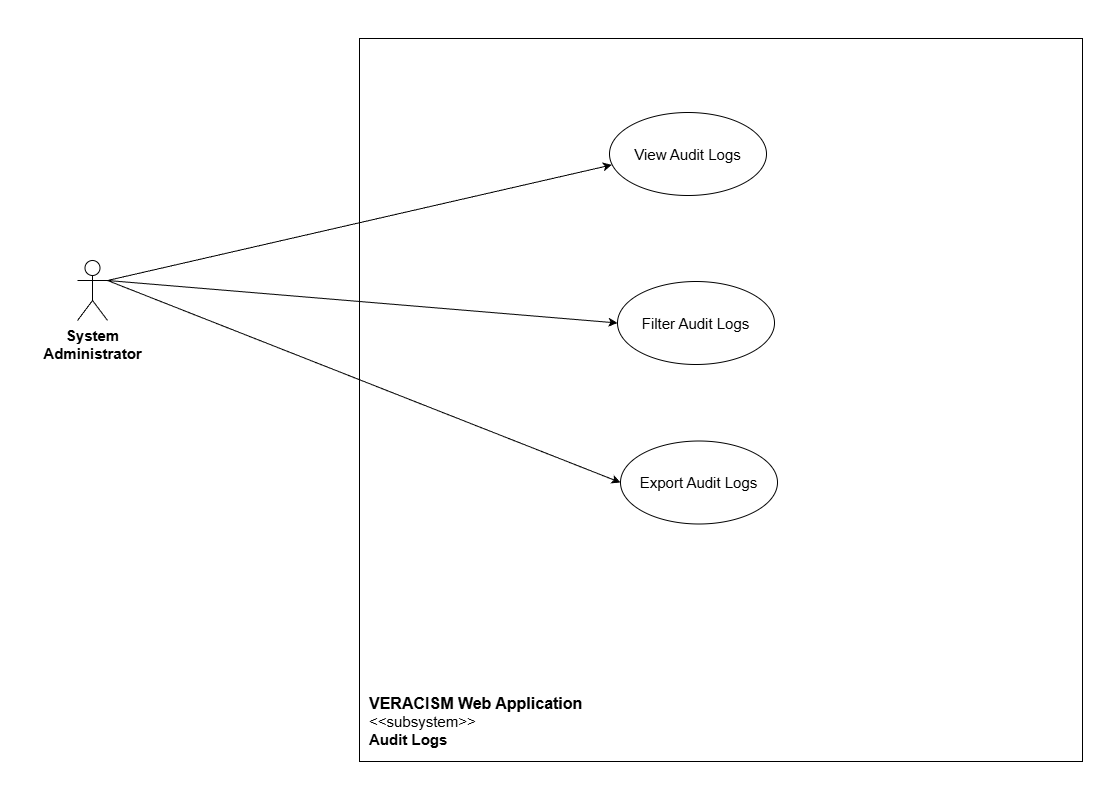
\includegraphics[height=0.43\textheight,keepaspectratio]{Texfiles/images/Use Case/Audit Logs.png}
        \caption{Use Case Diagram - Audit Logs}
        \label{fig:usecaseAuditLogs-diagram}
    \end{figure}

    \clearpage
    % Pair 5
    \begin{figure}[H]
        \centering
        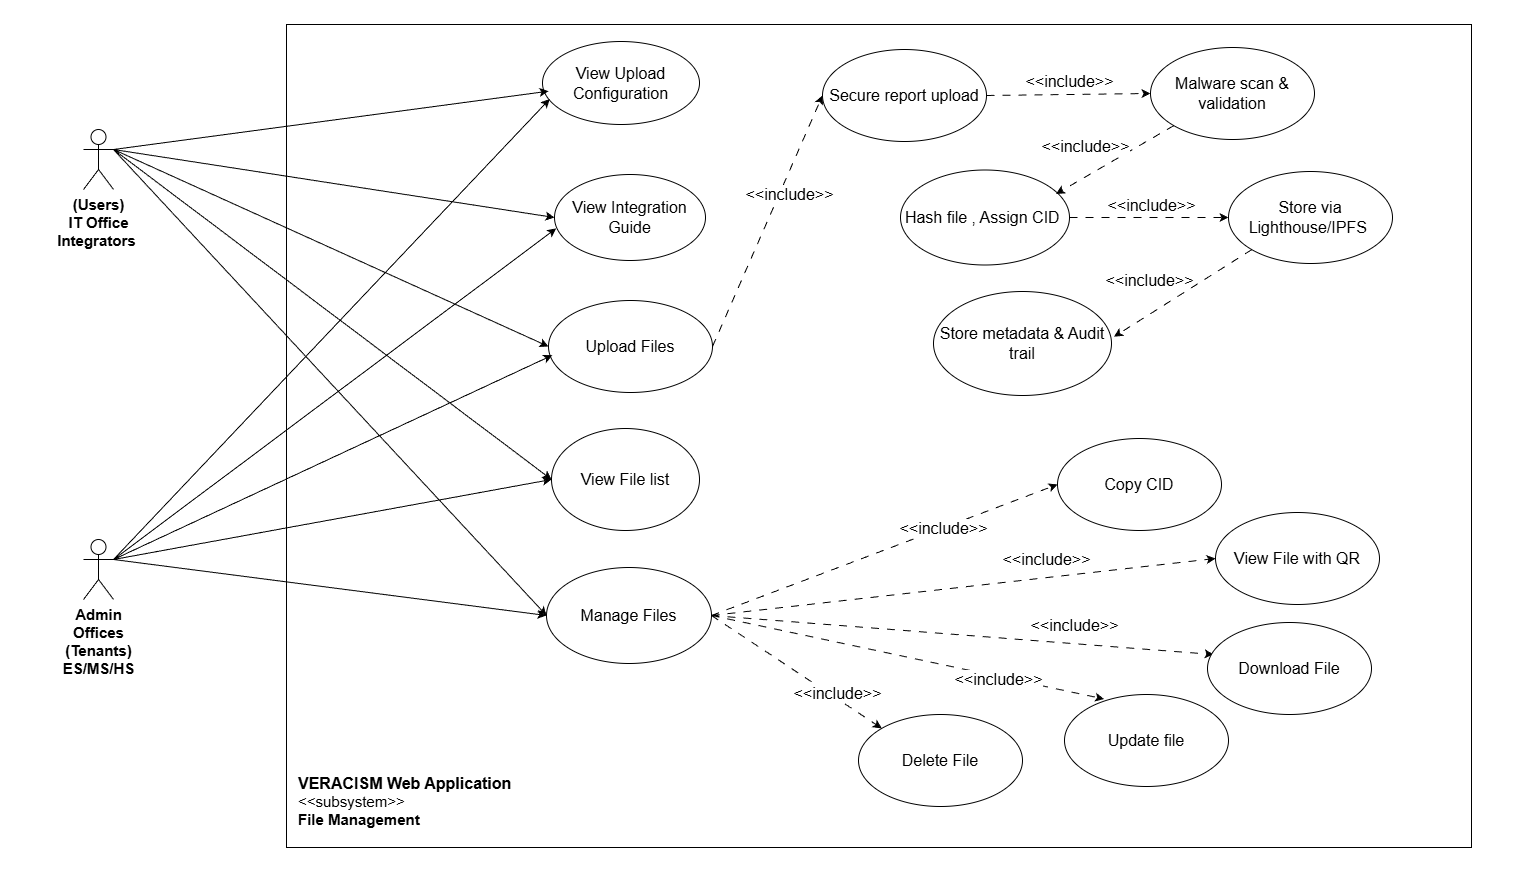
\includegraphics[height=0.43\textheight,keepaspectratio]{Texfiles/images/Use Case/File Management.png}
        \caption{Use Case Diagram - File Management}
        \label{fig:usecaseFileManagement-diagram}
    \end{figure}

    \begin{figure}[H]
        \centering
        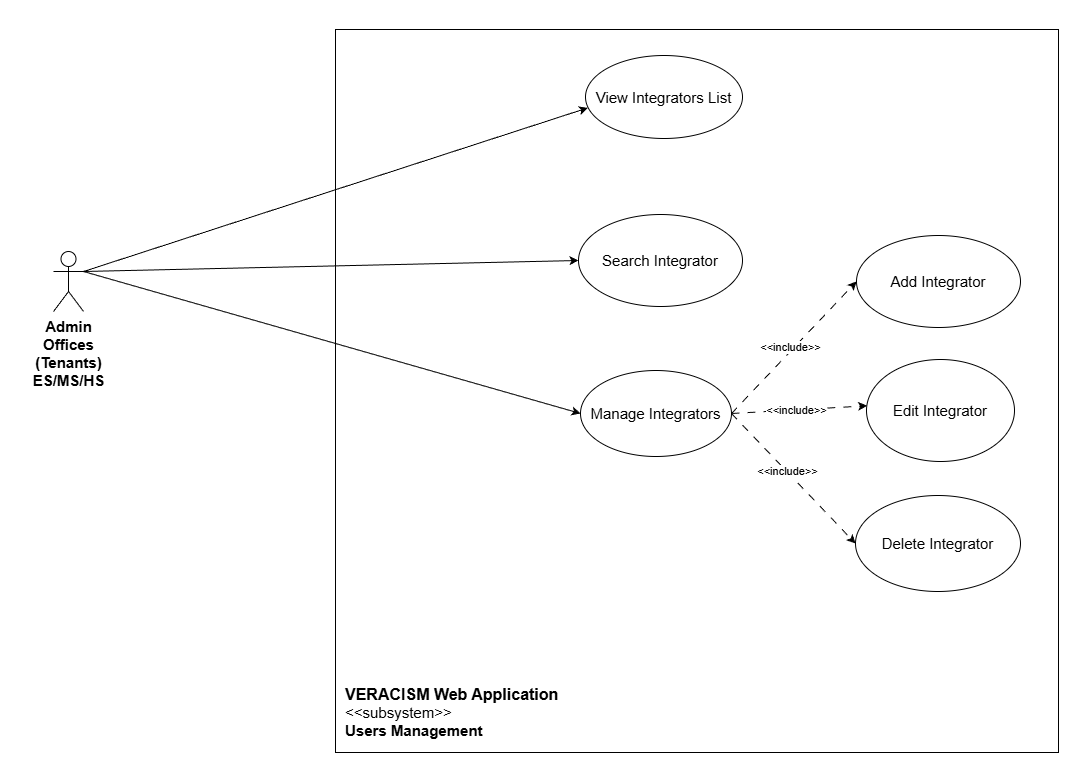
\includegraphics[height=0.43\textheight,keepaspectratio]{Texfiles/images/Use Case/Users Management.png}
        \caption{Use Case Diagram - Users Management}
        \label{fig:usecaseUsersManagement-diagram}
    \end{figure}

VERACISM is composed of several cooperating subsystems: the Landing Page and
Dashboard for high-level entry and monitoring, Tenants Management and Users
Management for multi-tenant administration, File Management for secure report
handling, and configuration-focused subsystems for Yara Rules Management,
ClamAV Management, API Keys Management, and Audit Logs. Each subsystem has its
own functional responsibilities and is used by specific actors: Admin, Tenants,
and Integrators. These actors interact with the system and show how
responsibilities are separated across modules.

The Landing Page and Dashboard subsystems
(Figures~\ref{fig:usecaseLandingPage-diagram} and
\ref{fig:usecaseDashboard-diagram}) present how Admin, Tenants, and
Integrators first interact with VERACISM. From the Landing Page, all roles can
view the homepage, read the API documentation, and sign in to the application.
The Dashboard diagram then shows how Admin and Tenants can see overall system
status: total uploads, passed scans, flagged scans, active tenants (for Admin),
and active integrators (for Tenants). Together, these diagrams provide a
high-level overview of how users enter the system and monitor its current
security and operational posture.

The Tenants Management and Users Management subsystems
(Figures~\ref{fig:usecaseTenantsManagement-diagram} and
\ref{fig:usecaseUsersManagement-diagram}) focus on multi-tenant control and
delegating integration responsibilities. The Tenants Management diagram shows
how the Admin views the tenant list and manages tenants through the included
use cases for adding, editing, and deleting tenants. This represents how
VERACISM onboards or offboards entire organizations. The Users Management
diagram shows how a Tenant user manages their own integrators: viewing the
integrator list, searching integrators, and using the included actions to add,
edit, or delete integrator accounts. These diagrams clarify how central
administration and tenant-level administration work together to control who
can integrate systems with VERACISM.

The Settings, Yara Rules Management, ClamAV Management, API Keys Management,
and Audit Logs subsystems
(Figures~\ref{fig:usecaseSettings-diagram},
\ref{fig:usecaseYaraRulesManagement-diagram},
\ref{fig:usecaseClamAVManagement-diagram},
\ref{fig:usecaseAPIKeysManagement-diagram}, and
\ref{fig:usecaseAuditLogs-diagram}) illustrate how security and configuration
are handled by the Admin. The Settings diagram summarizes the main
configuration areas: Yara rules, ClamAV, API keys, and viewing audit logs. The
Yara Rules Management diagram shows how the Admin views the ruleset list, tests
with samples, uploads new rulesets, and uses the included actions to disable or
delete specific rules. The ClamAV Management diagram shows how the Admin
monitors engine status, signature databases, scan statistics, and recent
activity, and then manages ClamAV by updating signatures, scheduling automatic
updates, running test scans, and viewing logs. The API Keys Management diagram
presents how the Admin views all API keys and uses the included actions to add,
delete, or refresh keys for integrated systems. The Audit Logs diagram shows
how the Admin can view, filter, and export audit logs to support traceability,
investigations, and compliance. Together, these diagrams describe how VERACISM
centralizes security and operational controls under a restricted Admin role.

The File Management subsystem (Figure~\ref{fig:usecaseFileManagement-diagram})
captures the core business flow for Tenants and Integrators. The diagram shows
how these roles view upload configuration and integration guides before sending
any files. The Upload Files use case represents the complete pipeline: secure
report upload, malware scanning and validation, hashing and CID assignment,
storage via Lighthouse/IPFS, and storing metadata and audit trail entries, each
modeled as an included use case. After upload, Tenants and Integrators can view
the file list and perform file management operations: copying CIDs, viewing
files with QR codes, downloading files, and, where permitted by policy,
updating or deleting files through the corresponding included use cases. This
diagram illustrates how VERACISM enforces a secure, traceable, and
content-addressed workflow for report files.

The use case diagrams give a clear map of how VERACISM works in practice. They
show how users enter the system, how tenants and integrators are controlled,
how security and configuration are maintained by Admins, and how reports are
uploaded, scanned, stored, and retrieved. This view helps identify the actors,
responsibilities, and interactions that must be built and tested so that the
platform remains secure, auditable, and aligned with ISM’s operational needs.


    

    \clearpage
\subsection{Sequence diagram – Upload Workflow}


    \begin{figure}[H]
        \centering
        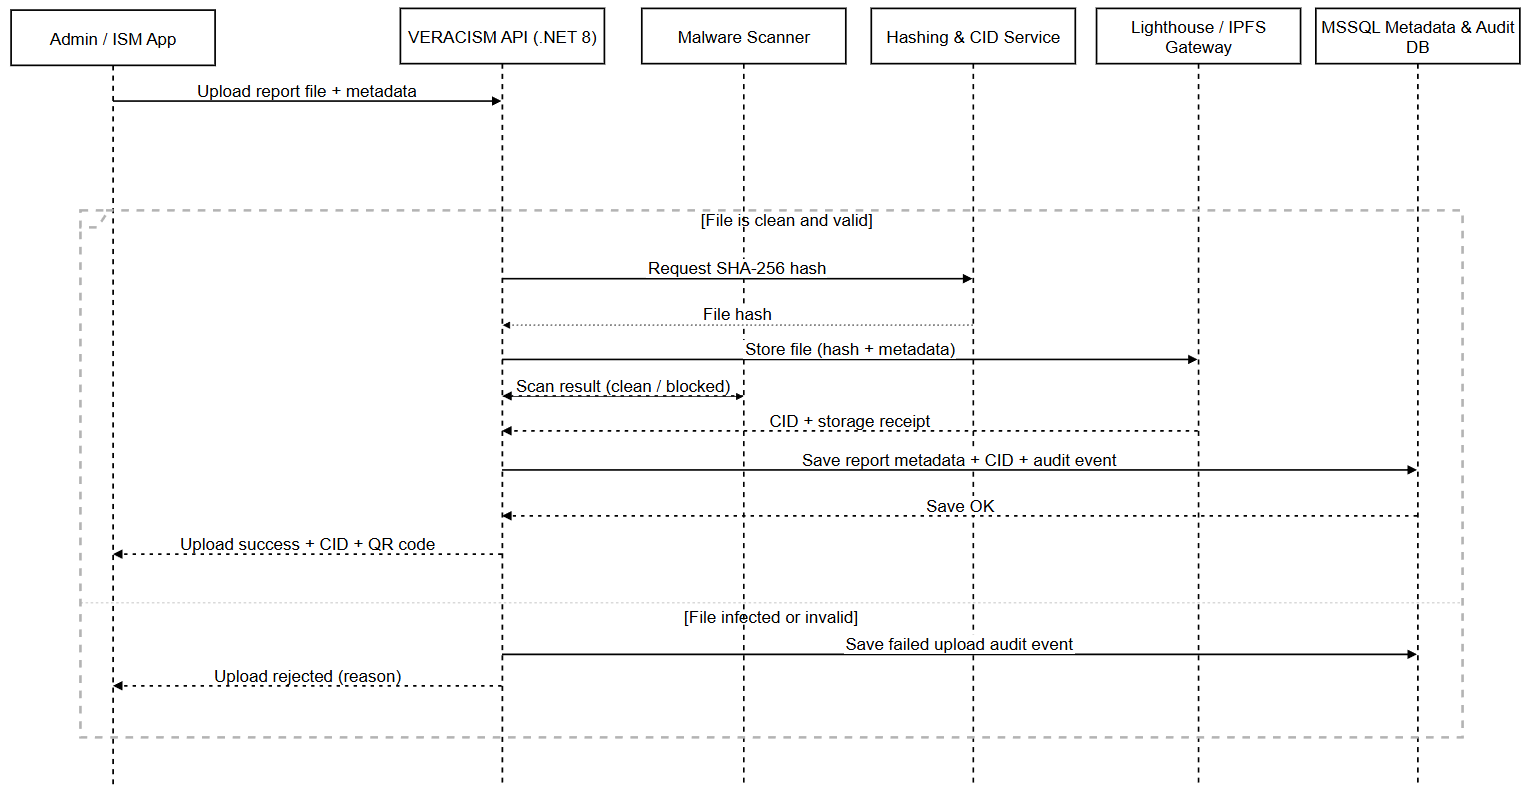
\includegraphics[height=250px,keepaspectratio]{Texfiles/images/Veracism - Upload.PNG}
        \caption{Sequence diagram – Upload Workflow}
        \label{fig:seq-upload-flow}
    \end{figure}

Figure~\ref{fig:seq-upload-flow} explains what happens to a report file from the
time an Admin or ISM system sends it to VERACISM until the system decides
to accept or reject it. The main lifelines are the Admin / ISM App, the
VERACISM API (.NET 8), the Malware Scanner, the Hashing and CID Service,
the Lighthouse / IPFS gateway, and the MSSQL metadata and audit database.
The diagram follows the file step by step so it is clear when security
checks run, when the hash and CID are created, when the file is pushed to
decentralized storage, and when audit records are written.

In Upload workflow the report file uploads 
together with its metadata to the VERACISM API. The API forwards the file
to the Malware Scanner, and once the file is considered clean and valid,
requests a SHA-256 hash from the Hashing and CID Service. After the hash
is returned, the API sends the file, hash, and metadata to Lighthouse /
IPFS for storage. Lighthouse returns the CID and storage receipt, and the
API saves the report metadata, CID, and an audit event in the MSSQL
database. When the save operation succeeds, the API responds to the
Admin / ISM App with an upload success message that includes the CID and
the QR code that can be printed on or attached to the report.

The diagram also covers the failure path when a file is infected or
invalid. In this case, the Malware Scanner returns a blocked or invalid
result, and the VERACISM API does not proceed to hashing or decentralized
storage. Instead, it records a failed upload audit event in MSSQL and
returns an “upload rejected” response to the Admin / ISM App together
with the reason. This makes sure that even rejected uploads are fully
traceable and that no unsafe or non-compliant files enter the permanent
storage workflow.



    \clearpage
\subsection{Sequence diagram – File Verification Workflow}


    \begin{figure}[H]
        \centering
        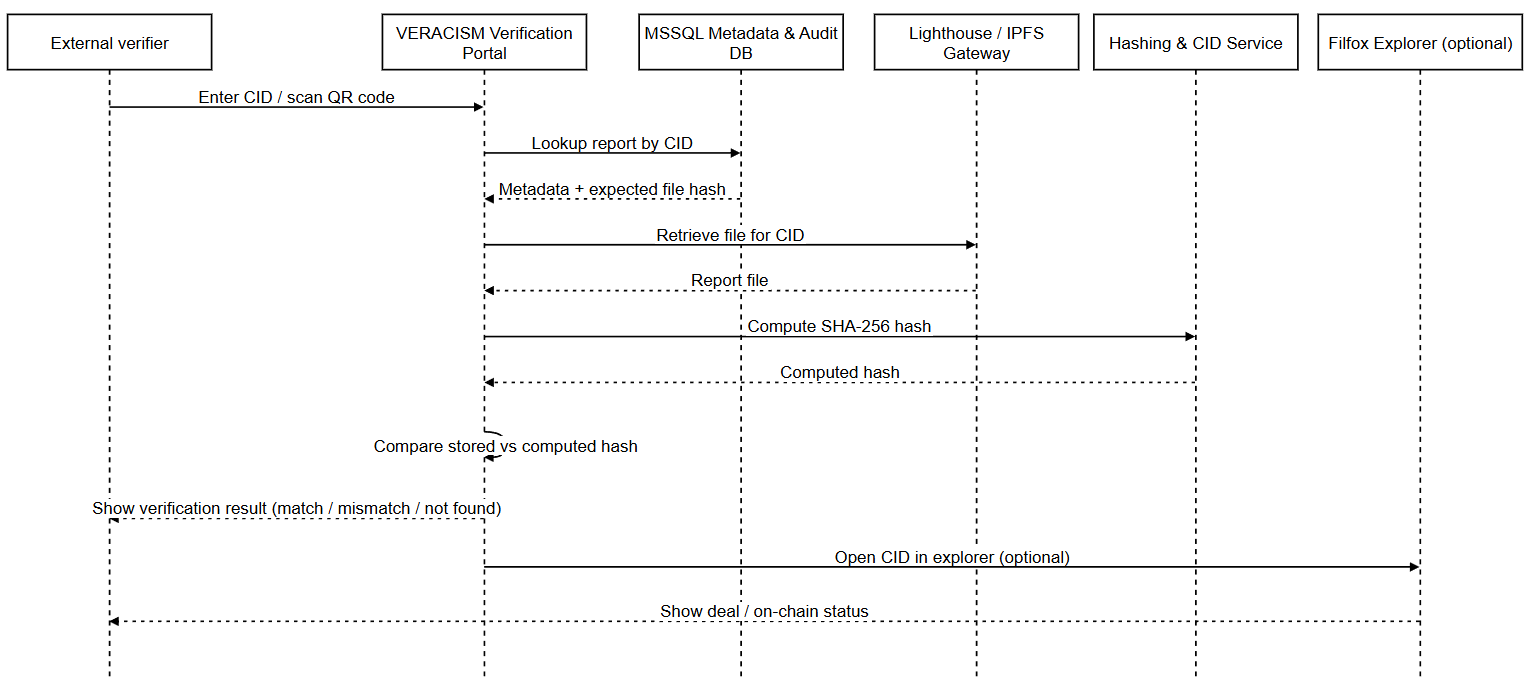
\includegraphics[height=220px,keepaspectratio]{Texfiles/images/Veracism - Verify.PNG}
        \caption{Sequence Diagram – File Verification Workflow}
        \label{fig:seq-verification-flow}
    \end{figure}

The Figure~\ref{fig:seq-verification-flow} focuses on the main participants in a
verification request started with a CID or QR code. The lifelines include
the External Verifier (for example a student, auditor, or educator), the
VERACISM Verification Portal, the MSSQL metadata and audit database, the
Lighthouse / IPFS gateway, the Hashing and CID Service, and a public
explorer such as Filfox. This context sets up the detailed flow of lookups,
file retrieval, and hash comparison described in the next steps.

In the normal verification flow, the External Verifier enters a CID in
the portal or scans a QR code printed on the report. The Verification
Portal sends a lookup request to MSSQL to find the matching report
metadata, including the expected file hash and basic report details. Once
the metadata is found, the portal asks the Lighthouse / IPFS gateway to
retrieve the file for the given CID. The gateway returns the report file,
which is then passed to the Hashing and CID Service.

The Hashing and CID Service computes a fresh SHA-256 hash of the retrieved
file and returns the computed hash to the portal. The portal compares this
computed hash with the stored hash from MSSQL. If they match, the portal
shows a “match” result along with key metadata so that the verifier can see
that the file has not changed since it was registered in VERACISM.
If the hashes differ or if the CID or report cannot be found, the
verification result is shown as “mismatch” or “not found,” clearly
indicating that integrity or availability cannot be confirmed.

In addition to this core flow, the External Verifier may also view deal or
on-chain status by opening the CID in a public explorer such as Filfox. In
this step, the portal provides a link to the explorer, which displays information about the storage
deal and other public evidence related to the CID. This extra
check strengthens transparency by allowing verifiers to confirm VERACISM’s
internal records against independent decentralized storage evidence for the
same content.


    \clearpage
    
\subsection{Database diagram}

    \begin{figure}[H]
        \centering
        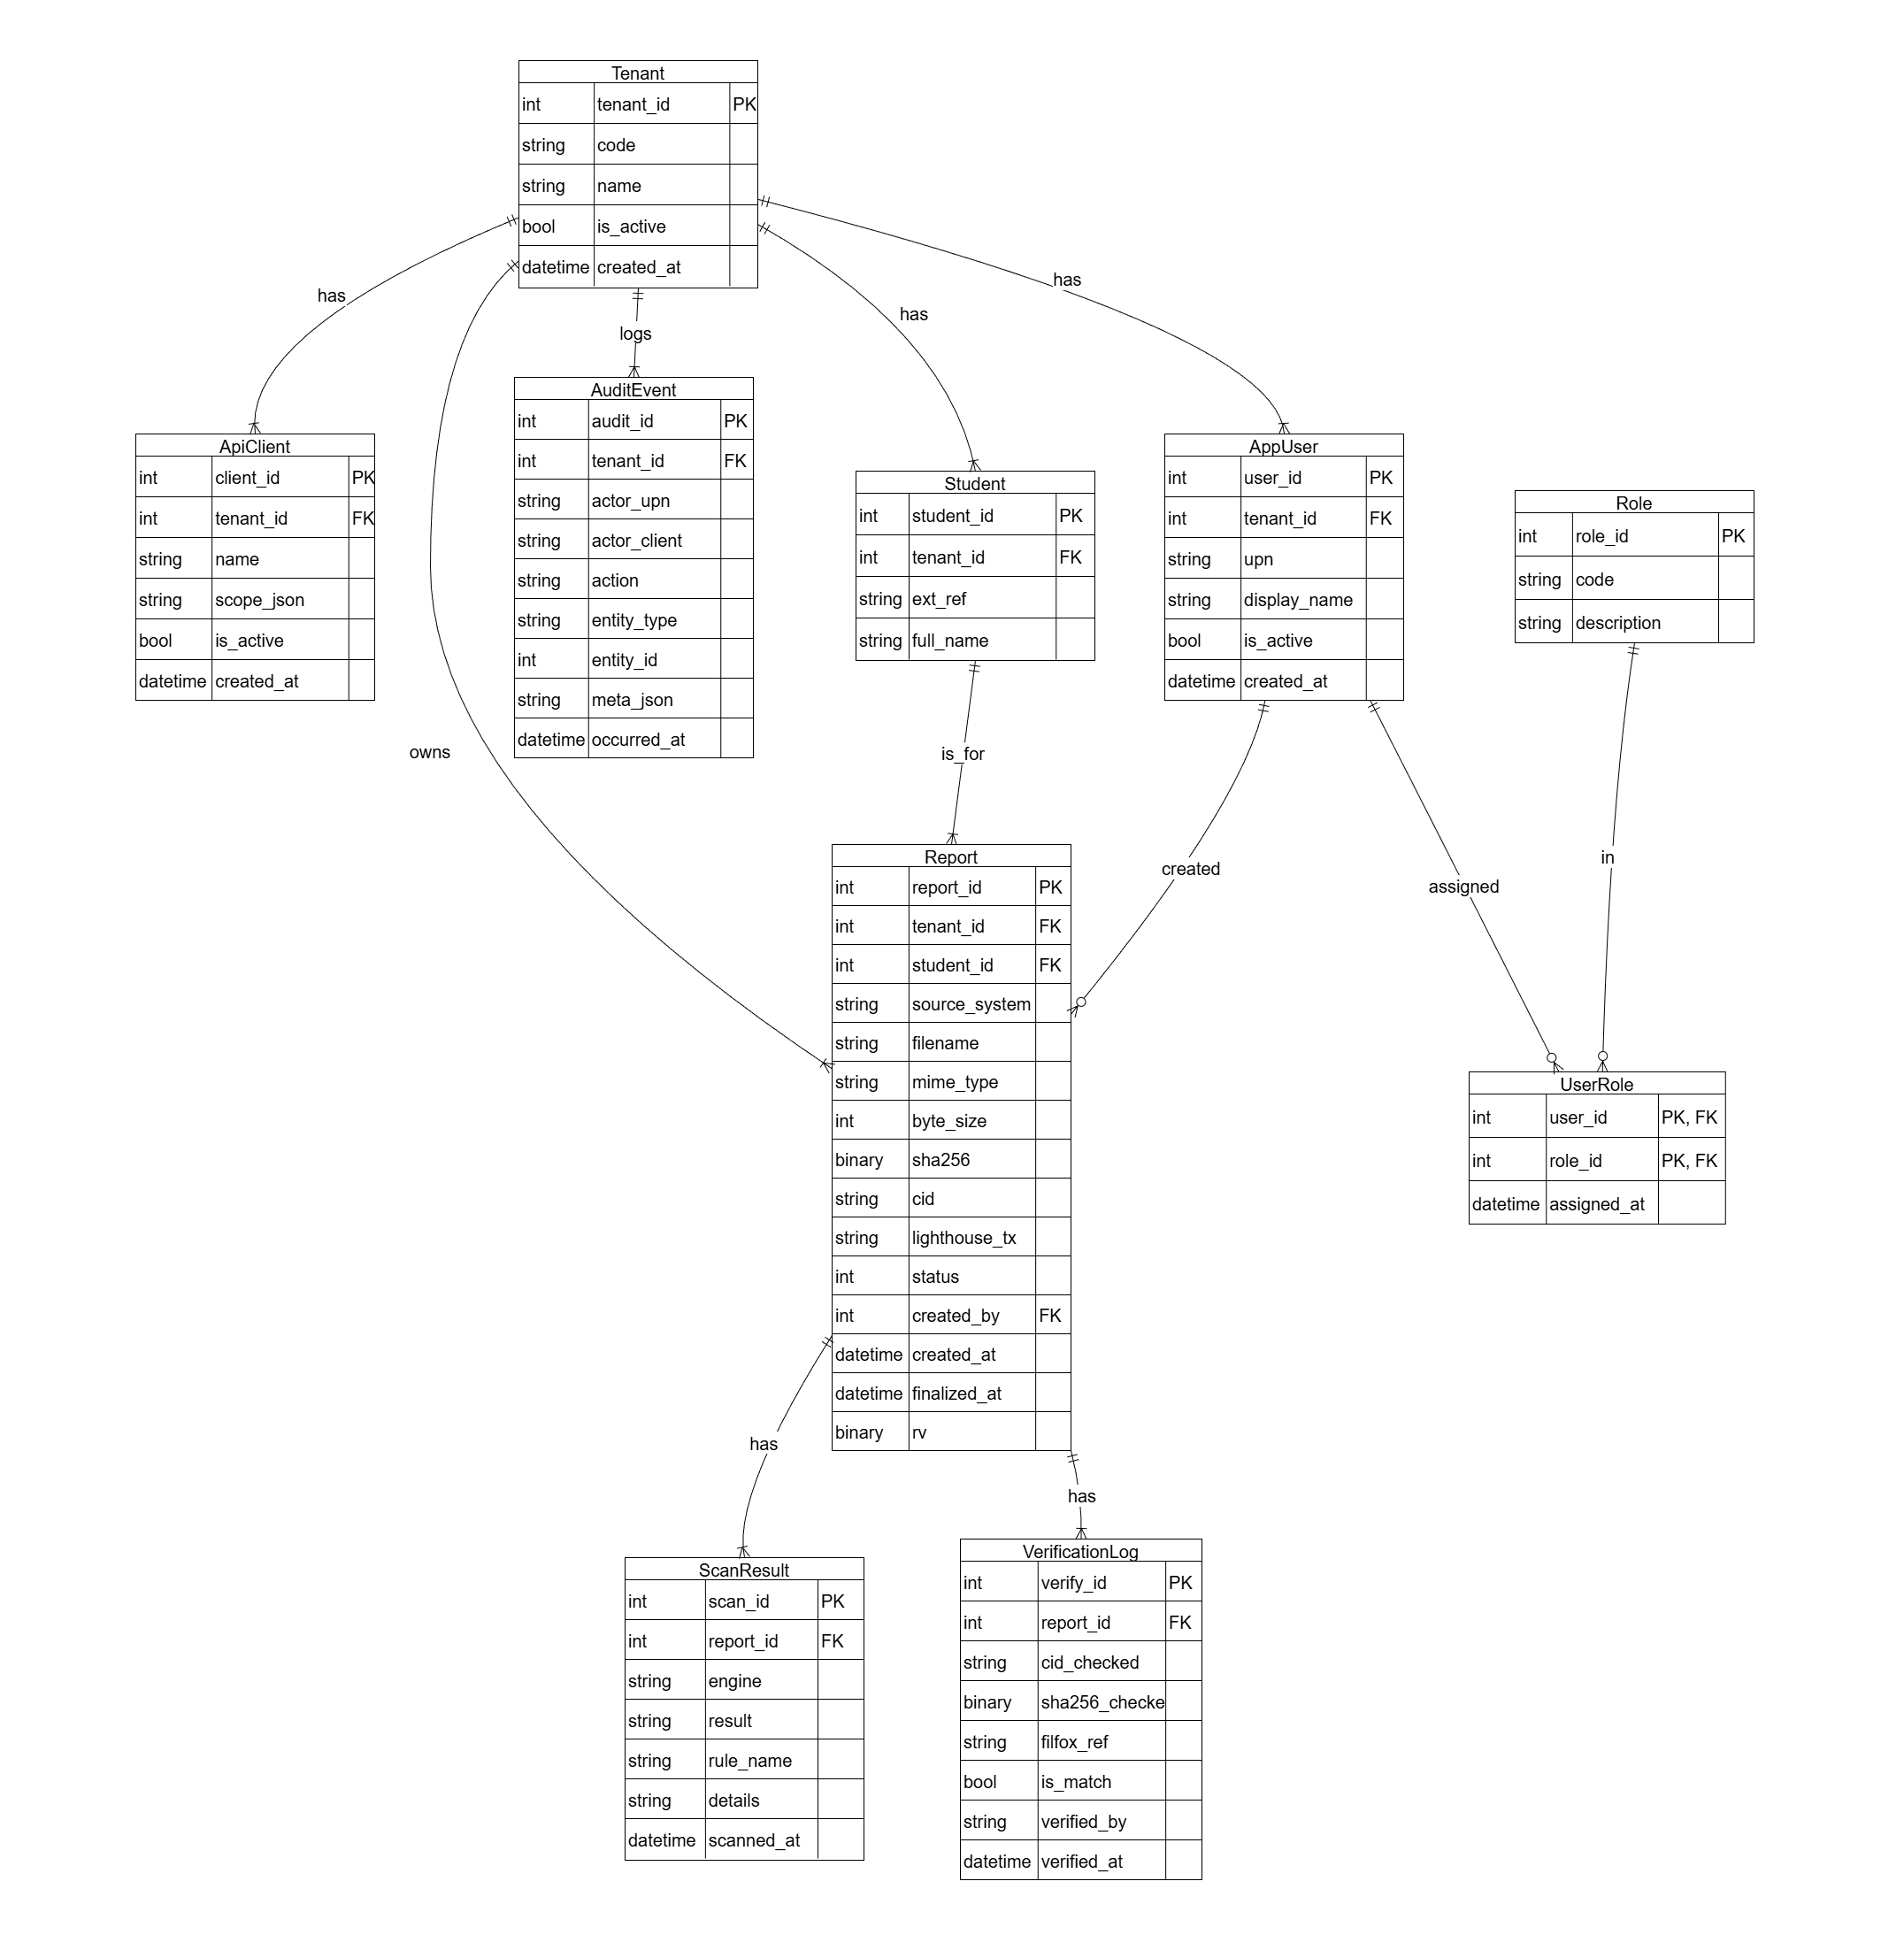
\includegraphics[height=.8\textheight,keepaspectratio]{Texfiles/images/Veracism - ERD.png}
        \caption{Database diagram}
        \label{fig:seq-database-diagram}
    \end{figure}

The Figure~\ref{fig:seq-database-diagram} follows the data model defined in the SRS and is
implemented in MSSQL. The ERD groups data into a small set of focused
entities that capture tenants, users, reports, security scans, and
verification activity, with clear relationships between them.

At the center of the model is the \textbf{\texttt{Tenant}} table. Each row
represents one organization (for example, ISM itself or a future partner)
and holds identifiers, codes, and status flags. A single tenant owns all
other core records in the system: its reports, API clients, users,
students, and audit events. This makes it easy to enforce isolation and
filter every query by \texttt{tenant\_id}.

The \textbf{\texttt{AppUser}} table stores human users such as admins and
tenant operators. Each user belongs to exactly one tenant and has fields
for login identity, display name, status, and creation time. User
permissions are modeled through the \textbf{\texttt{Role}} and
\textbf{\texttt{UserRole}} tables. \texttt{Role} contains the list of
available roles (for example, TenantAdmin, Integrator, or Viewer), while
\texttt{UserRole} is a junction table that assigns one or more roles to a
given user within a tenant. In the ERD, an \texttt{AppUser} can have many
\texttt{UserRole} rows, and each \texttt{UserRole} links back to exactly
one \texttt{Role}. This structure supports flexible RBAC with minimal
duplication.

Machine-to-machine integrations are represented by the
\textbf{\texttt{ApiClient}} table. Each API client belongs to a tenant and
is identified by a client id, name, and scope. Active flags and timestamps
help operations teams track which integrations are still in use. In the
diagram, tenants can own many API clients, and those clients can be linked
to the reports they create or manage, so that VERACISM can distinguish
between human-triggered and system-triggered activity.

Student-related information is modeled through the
\textbf{\texttt{Student}} table. Each student belongs to one tenant and
stores identifiers (such as \texttt{student\_id} and \texttt{ext\_ref})
and a full name. The \textbf{\texttt{Report}} table then links directly to
\texttt{Student} via \texttt{student\_fk}. Each \texttt{Report} row
represents a finalized report file and includes the tenant id, the source
system, filename, MIME type, file size, SHA-256 hash, CID, Lighthouse
transaction reference, status, and timestamps for creation and finalization.
Foreign keys such as \texttt{created\_by\_fk} tie reports back to the user
or integration that submitted them. In the ERD, a single student can be
associated with many reports, but each report points to exactly one
student and one tenant.

Security scan results are captured in the \textbf{\texttt{ScanResult}}
table. Each scan record belongs to one report and records the scan engine
(ClamAV, YARA, or other), the result (clean, infected, blocked), the rule
name, details, and the scan timestamp. The relationship is one-to-many:
each report can have zero or more scan results (for example, if it was
rescanned after a rule update), but each scan result is linked to a single
report. This makes it easy to review the full history of scanning decisions
for any report.

Verification activity is logged in the \textbf{\texttt{VerificationLog}}
table. Each entry records an individual verification event, including the
report id, the CID that was checked, the SHA-256 hash observed at
verification time, any external references such as a Filfox URL, whether
the result was a match or mismatch, who performed the verification, and
when it occurred. As with scan results, the relationship is one-to-many:
a report can have multiple verification log entries over time, but each
verification log refers to a single report. This allows auditors to see
how often and by whom a report has been checked.

Operational and security actions across the system are captured by the
\textbf{\texttt{AuditEvent}} table. Each audit event belongs to a tenant
and stores an event id, actor information (user, API client, or system),
the action name, the entity type and id that were affected, a JSON payload
for detailed metadata, and the time the event occurred. Tenants can have
many audit events, and events can reference reports, configuration items,
or other domain entities. This design supports an immutable, searchable
audit trail for compliance and incident investigation.

The relationships in the ERD enforce a clear structure: each
tenant owns its users, API clients, students, reports, scan results,
verification logs, and audit events. Reports sit at the core of the data
model and are linked outward to students, creators, security scans,
verifications, and audit history, so that any report can be traced from
its origin through scanning, storage, and verification activities.



    \clearpage
\subsection{Deployment diagram}

 \begin{figure}[H]
        \centering
        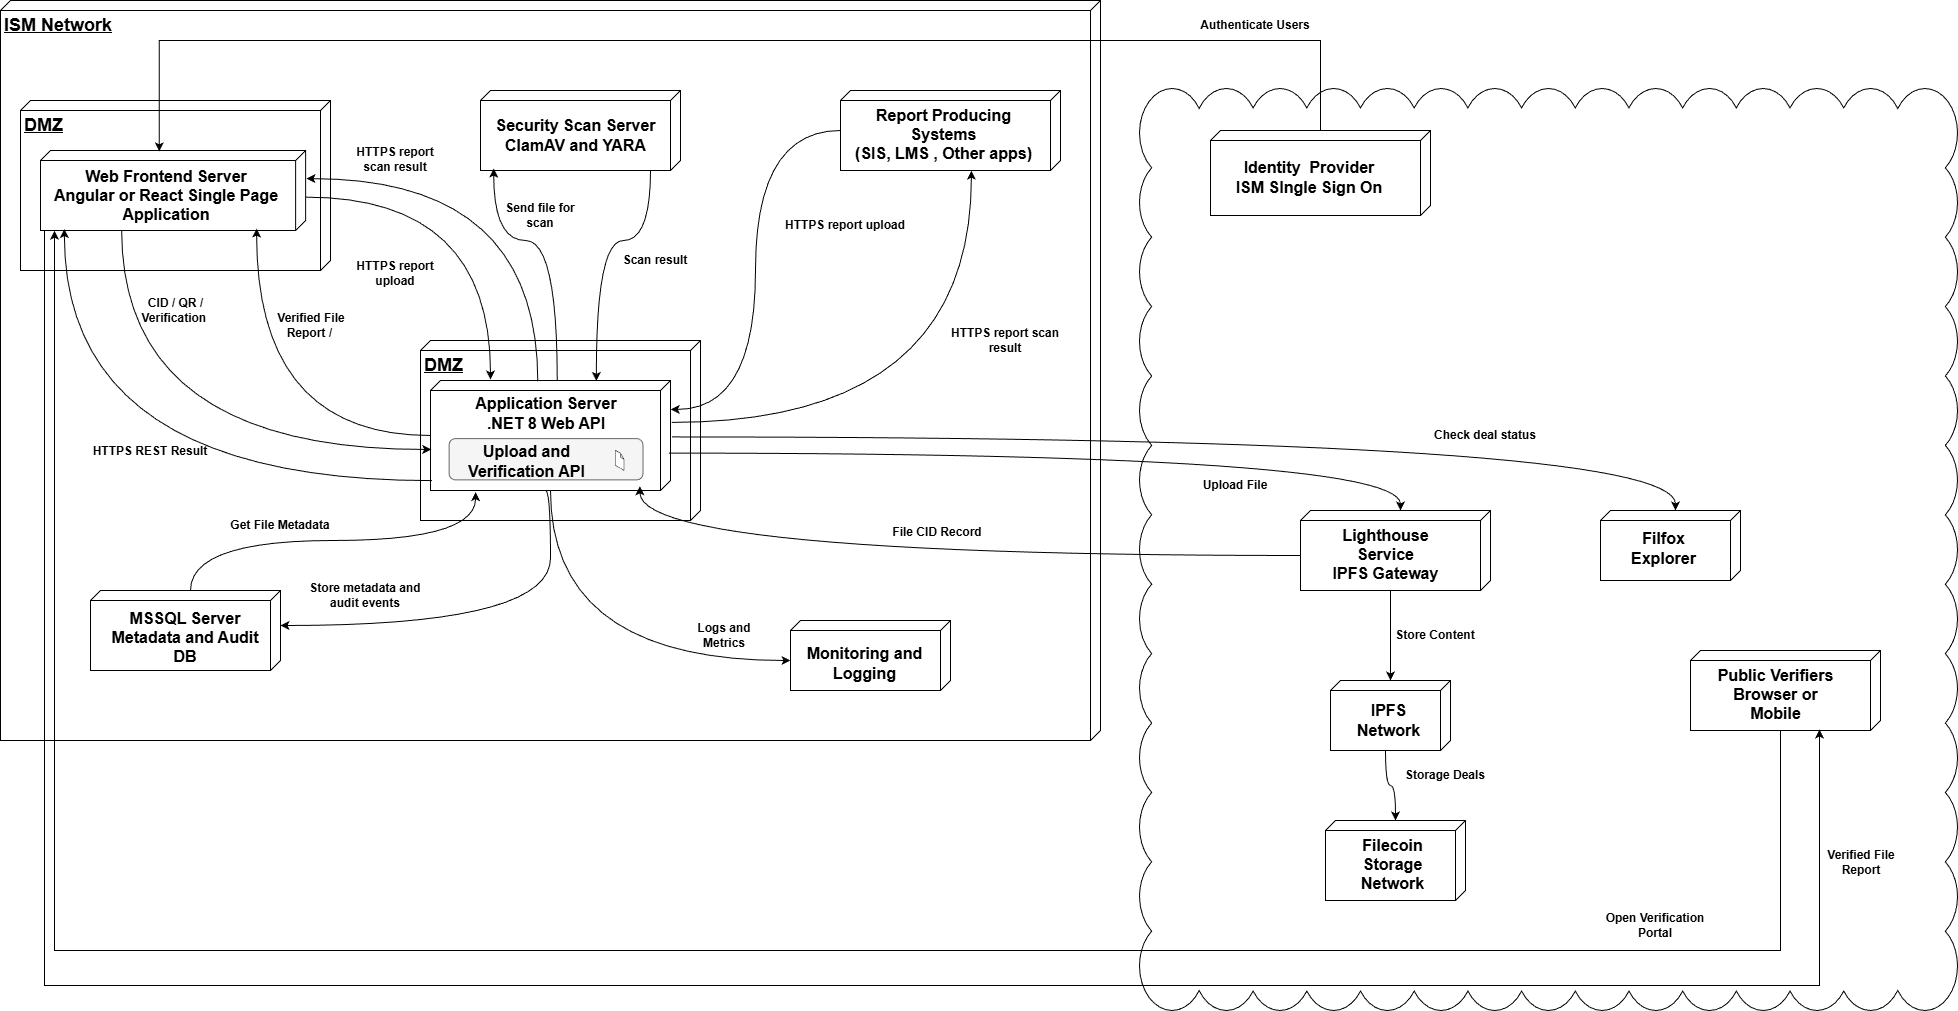
\includegraphics[height=0.38\textheight,keepaspectratio]{Texfiles/images/Veracism Deployment Diagram.png}
        \caption{Deployment diagram}
        \label{fig:deployment-diagram}
    \end{figure}

Figure~\ref{fig:deployment-diagram} places each VERACISM component either inside the ISM
network or in external services and maps the connections between them. On
the ISM side are the web frontend, the .NET 8 application server, the
security scan server, the MSSQL metadata and audit database, and the
monitoring and logging stack. On the external side are the Lighthouse IPFS
gateway, the IPFS and Filecoin networks, Filfox, the ISM identity
provider, and public verifiers using a browser or mobile device.

Within the ISM network, users and report-producing systems (SIS, LMS, and
other apps) first connect to the Web Frontend Server in the DMZ. This
frontend serves the Angular or React single-page application, which then
calls the Application Server (.NET 8 Web API) over HTTPS. The application
server exposes the upload and verification APIs and is placed in its own
DMZ segment so that database and monitoring servers stay behind an
additional boundary.

When a report is uploaded, the Application Server forwards the file to the
Security Scan Server running ClamAV and YARA. After scanning, the
application stores metadata and audit events in the MSSQL Server and sends
logs and metrics to the Monitoring and Logging stack. For accepted files,
the application also calls the Lighthouse IPFS gateway over HTTPS to upload
the content, receive the CID, and record the storage details back into the
MSSQL database.

User identity and sign-in are handled by the ISM Single Sign-On identity
provider, which authenticates users and issues tokens that the Web
Frontend and Application Server can validate. This keeps passwords and
authentication logic in one place while letting VERACISM focus on upload,
storage, and verification.

On the decentralized side, Lighthouse writes the file to the IPFS network
and arranges storage deals on the Filecoin storage network. Public verifiers
(such as students, parents, or auditors) access the VERACISM verification
portal from a browser or mobile device. The portal talks back to the
Application Server to fetch metadata and to the Lighthouse/IPFS gateway to
retrieve content for hashing. If a verifier wants more detail about storage
deals, the system can also open the CID in Filfox, which is shown as an
optional external component.

This deployment view makes it clear which components stay inside the ISM
network and which ones sit outside. It also shows the path a report
follows: from upload in the frontend, through scanning and storage in the
application and database layer, out to Lighthouse, IPFS, and Filecoin, and
back again when someone verifies a report from the portal. By reading the
diagram, a reader can see how VERACISM keeps internal systems protected
while still letting external users verify reports through public
decentralized services.
   

    \clearpage
    
\subsection{Implementation timeline}

\begin{figure}[H]
    \centering
    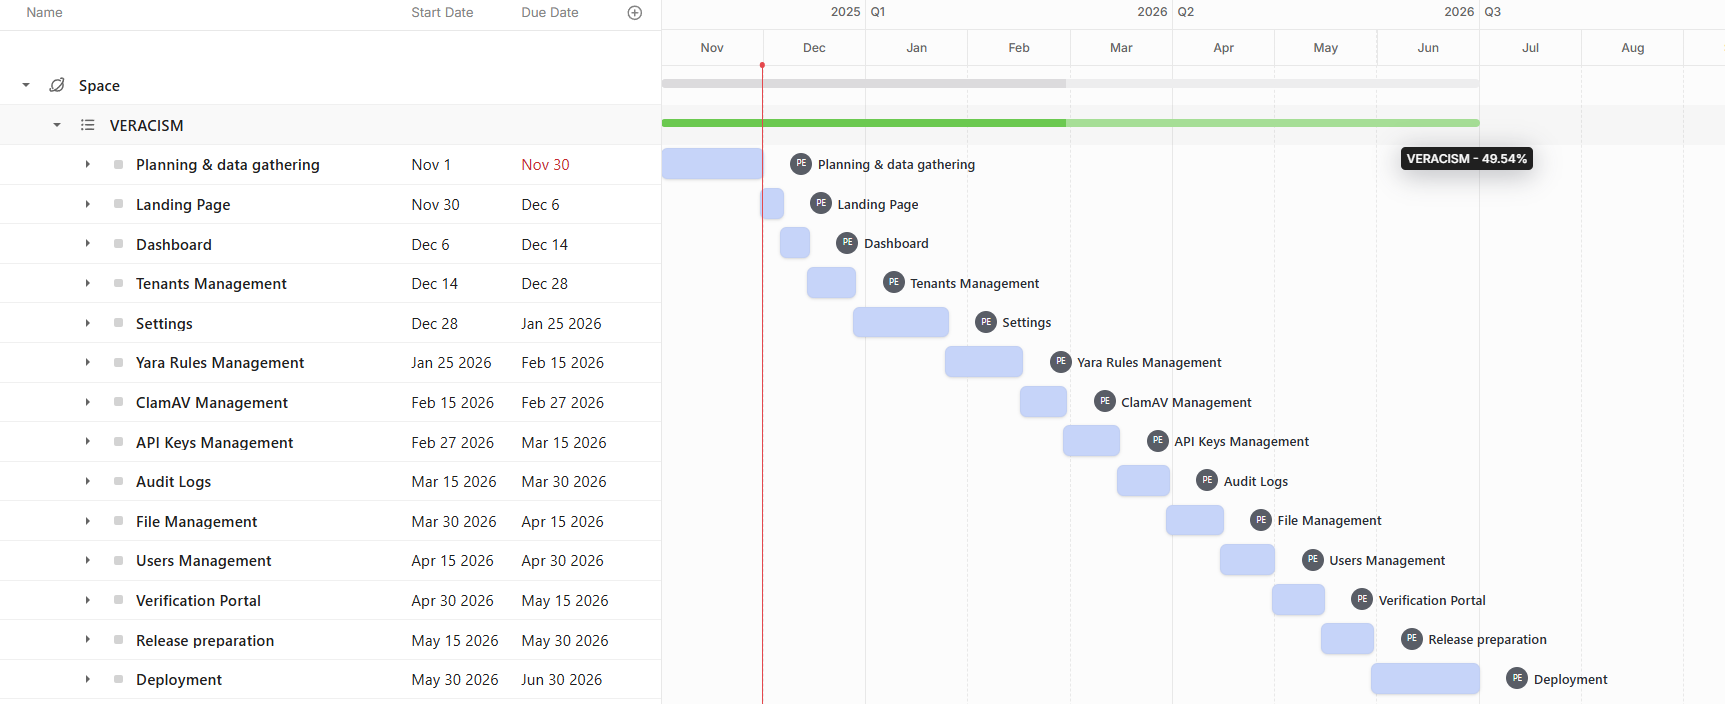
\includegraphics[height=0.32\textheight,keepaspectratio]{Texfiles/images/Veracism -Gantt Chart.png}
    \caption{Implementation Timeline}
    \label{fig:seq-implementation-timeline}
\end{figure}

Figure~\ref{fig:seq-implementation-timeline} shows the work laid out month by month from November 2025 to June 2026. The schedule follows a DevSecOps lifecycle that begins with planning and data gathering, then moves through each feature subsystem (Landing Page, Dashboard, Tenants Management, Settings, Yara Rules, ClamAV, API Keys, Audit Logs, File Management, Users Management, and the Verification Portal), and ends with release preparation and deployment. Each bar corresponds to one subsystem from the SRS and the use case models. The security focused modules are positioned ahead of the core file and user workflows and the production rollout activities.

Progress on the chart indicates that VERACISM is currently about \textbf{49.54\%} complete. Planning, Landing Page, and Dashboard are finished. Tenants, Settings, and the security modules are the next active blocks. The remaining items (File Management, Users Management, Verification Portal, release preparation, and deployment) complete the functional and non functional requirements before go live.

\subsubsection{Implementation and testing roadmap}

The implementation and testing roadmap organized VERACISM validation across
the Development, UAT, and Production environments. In the Development
environment, each subsystem is verified as it is built through unit tests, API
contract checks, and security controls that confirm correct behavior before
changes are promoted. The UAT environment is configured to mirror the school
operating context, including tenant setup, role-based access, realistic report
samples, and the same upload and verification paths that registrars, students,
and external verifiers will follow. This stage prioritizes end-to-end school
workflows and produces evidence such as logs, audit events, verification
results, and captured test artifacts that demonstrate conformance to required
behaviors. After UAT sign-off, the Production environment is used only for
controlled release and post-deployment verification to confirm that
configuration, monitoring, logging, and security gates operate correctly under
live conditions. Across these stages, functional testing, integration testing,
performance testing, user acceptance testing, and security testing are scheduled
as part of the overall validation process, while the detailed assessment
methodology for each testing area is presented in the Project Assessment
section.

\begin{table}[H]
  \centering
  \smalltable
  \footnotesize

  {%
  \setlength{\tabcolsep}{8pt}% horizontal padding
  \renewcommand{\arraystretch}{1.4}% vertical padding

  \begin{tabular}{|>{\raggedright\arraybackslash}p{0.30\textwidth}|
                  >{\raggedright\arraybackslash}p{0.22\textwidth}|
                  >{\raggedright\arraybackslash}p{0.40\textwidth}|}
    \hline
    \textbf{Testing stage} & \textbf{Schedule} & \textbf{Focus and coverage} \\
    \hline\hline

    Functional testing &
    Nov 2025 to Apr 2026 &
    End to end functional tests across modules and API endpoints. Verifies that core features work as intended, including file upload processing, file validation, malware scanning, hashing, CID generation, metadata storage, and access control behavior based on RBAC and ABAC rules. \\
    \hline

    Integration testing &
    Feb 2026 to May 2026 &
    End-to-end flows across the API, MSSQL, Lighthouse/IPFS, and the verification portal using realistic report samples and test tenants. Confirms that subsystems behave correctly when combined. \\
    \hline

    Security testing &
    Mar 2026 to May 2026 &
    Vulnerability scanning and manual security testing aligned with the institutional VAPT process. Findings are fixed and re-tested before go-live. \\
    \hline

    Performance testing &
    Apr 2026 to May 2026 &
    Response time and concurrency tests for upload and verification to confirm service level targets under expected operating load. \\
    \hline

    User acceptance testing &
    May 2026 &
    Role-based testing with the System Administrator, Administration Offices (registrars), students, and external verifiers using scripted tasks derived from the system requirements and acceptance criteria. \\
    \hline

  \end{tabular}
  }% end local spacing changes

  \captionsetup{type=table}
  \caption{Testing stages and schedule for VERACISM}
  \label{tab:testing-stages-schedule}
\end{table}

\subsubsection{User acceptance testing timeline}

\begin{table}[H]
  \centering
  \smalltable
  \footnotesize

  {%
  \setlength{\tabcolsep}{8pt}% horizontal padding
  \renewcommand{\arraystretch}{1.4}% vertical padding

  \begin{tabular}{|>{\raggedright\arraybackslash}p{0.22\textwidth}|
                  >{\raggedright\arraybackslash}p{0.20\textwidth}|
                  >{\raggedright\arraybackslash}p{0.22\textwidth}|
                  >{\raggedright\arraybackslash}p{0.30\textwidth}|}
    \hline
    \textbf{Phase} & \textbf{Dates (2026)} & \textbf{User roles} & \textbf{Scope and outputs} \\
    \hline\hline
    UAT setup and briefing &
    May 4 to May 6 &
    System admin, IT office, registrar lead &
    Accounts issued, test tenants created, test data loaded, task scripts distributed, defect log format agreed. \\
    \hline
    Registrar UAT &
    May 7 to May 11 &
    Registrars (Administration Offices) &
    Upload workflow, status tracking, dashboard views, audit log review, and verification checks using issued reports and assigned CIDs. \\
    \hline
    Student UAT &
    May 12 to May 13 &
    Students &
    QR access, verification result screen comprehension, metadata summary review, and reporting of unclear messages or steps. \\
    \hline
    External verifier UAT &
    May 14 to May 18 &
    External verifiers (auditors or partner schools) &
    QR scan to verification result, CID entry verification, failure messaging for unavailable content, and repeat checks from different networks. \\
    \hline
    End-to-end UAT and sign-off run &
    May 19 to May 21 &
    All roles &
    Full journey from report upload to verification, including negative tests for tampered files and unavailable deals, then sign-off decisions. \\
    \hline
    Fix and retest window &
    May 22 to May 29 &
    IT office, registrar lead &
    Retest of defects, regression run, evidence capture, final acceptance sign-off. \\
    \hline
  \end{tabular}
  }% end local spacing changes

  \captionsetup{type=table}
  \caption{User acceptance testing timeline for VERACISM}
  \label{tab:uat-schedule}
\end{table}

UAT is scheduled while Users Management and the Verification Portal are available for end-to-end workflows, with closure before release preparation and deployment.

